\documentclass{article}
\usepackage[utf8]{inputenc}
\usepackage{graphicx}
\graphicspath{ {images/} }
\usepackage{multicol}
\setlength{\columnsep}{2cm}
%\oddsidemargin=0pt % отступ от левого края
%\topmargin=-1.5cm % отступ от верхнего края

\documentclass[12pt]{article}
\usepackage[cp1251]{inputenc}
\usepackage[russian]{babel}
\begin{document}

\begin{titlepage}
	\centering
	{\scshape\LARGE Московский физико-технический институт \par}
	\vspace{3cm}
	{\scshape\Large Лабораторная работа по курсу\\ Вакуумная электроника \par}
	\vspace{1cm}
	{\huge\bfseries Методы получения высокого вакуума \par}
	\vspace{1cm}
	%{\Large\itshape John Birdwatch\par}
	\vfill
\begin{flushright}
	{\large выполнили студенты 653 группы ФФКЭ}\par
	\vspace{0.3cm}
	{\LARGE Агафонов Владислав}\\
	{\LARGE Карпова Татьяна} %\textsc{Brown}
\end{flushright}

	\vfill

% Bottom of the page
Долгопрудный, 2017 г.
\end{titlepage}
\newpage

\tableofcontents


\section{Цель работы}
\begin{enumerate}
    \item Ознакомиться с принципами работы вакуумной техники: пластинчато-роторного насоса, турбомолекулярного насоса, ионизационного, ёмкостного и терморезистивного вакуумметров.
    \item Ознакомиться с методами вакуум-ных расчётов, найти зависимость величины газового потока в системе от давления.
    \item Определить производительность турбомолекулярного насоса.
    \item Рассчитать объем рабочей камеры.
\end{enumerate}

\section{Лабораторная установка}

Лабораторная установка предназначена для ознакомления с основными приборами вакуумной техники: насосами, манометрами, измерителями расхода газа. Схема установки представлена на рисунке 1.
\begin{figure}[h]
    \centering
    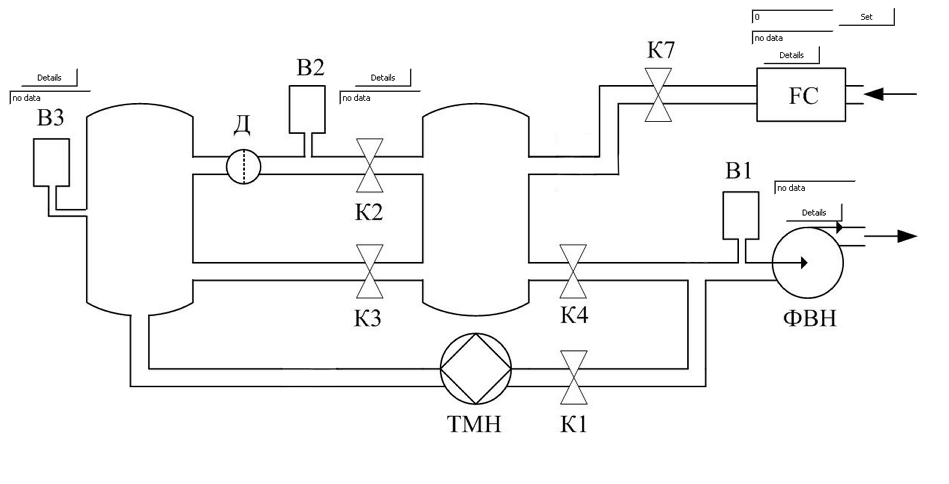
\includegraphics[width=\textwidth]{facility.PNG}
    \caption{Схема лабораторной установки}
    \label{fig:vac}
\end{figure}

На схеме обозначены: \\
$B_1$ - вакуумметр ёмкостной\\
$B_2$ - вакуумметр терморезисторный\\
$B_3$ - вакуумметр ионизационный\\
$K_1$ - кран турбомолекулярного насоса\\
$K_3$ - высоковакуумная заслонка\\
$K_4$ - форвакуумная заслонка\\
$K_2, K_7$ - коммутационные краны\\
Д - диафрагма\\
FC - регулятор газового потока (flow controller)\\
ТМН - турбомолекулярный насос\\
ФВН - форвакуумный насос\\

\section{Выполнение работы}
\subsection{Измерение давления в форвакуумной части установки}
\begin{enumerate}
    \item Включаем компьютер, подаём питание на установку
    \item Все краны кроме К1 переводим в открытое положение, кран К1 остаётся закрытым
    \item Включаем ёмкостной (В1) и терморезисторный (В2) вакуумметры, включаем регулятор газового потока (FC), устанавливаем поток газа 0 sccm. Дожидаемся стабилизации показаний датчика регулятора газового потока. Поток стабилизировался на значении примерно 1.7 sccm и не опускается до нуля. 
    \item Включаем форвакуумны насос и снимаем показания ёмкостного и терморезисторного вакуумметров. Зависимость показаний давления в орвакуумной части от времени показана на графике 1.
\end{enumerate}

\begin{figure}[h]
    \centering
    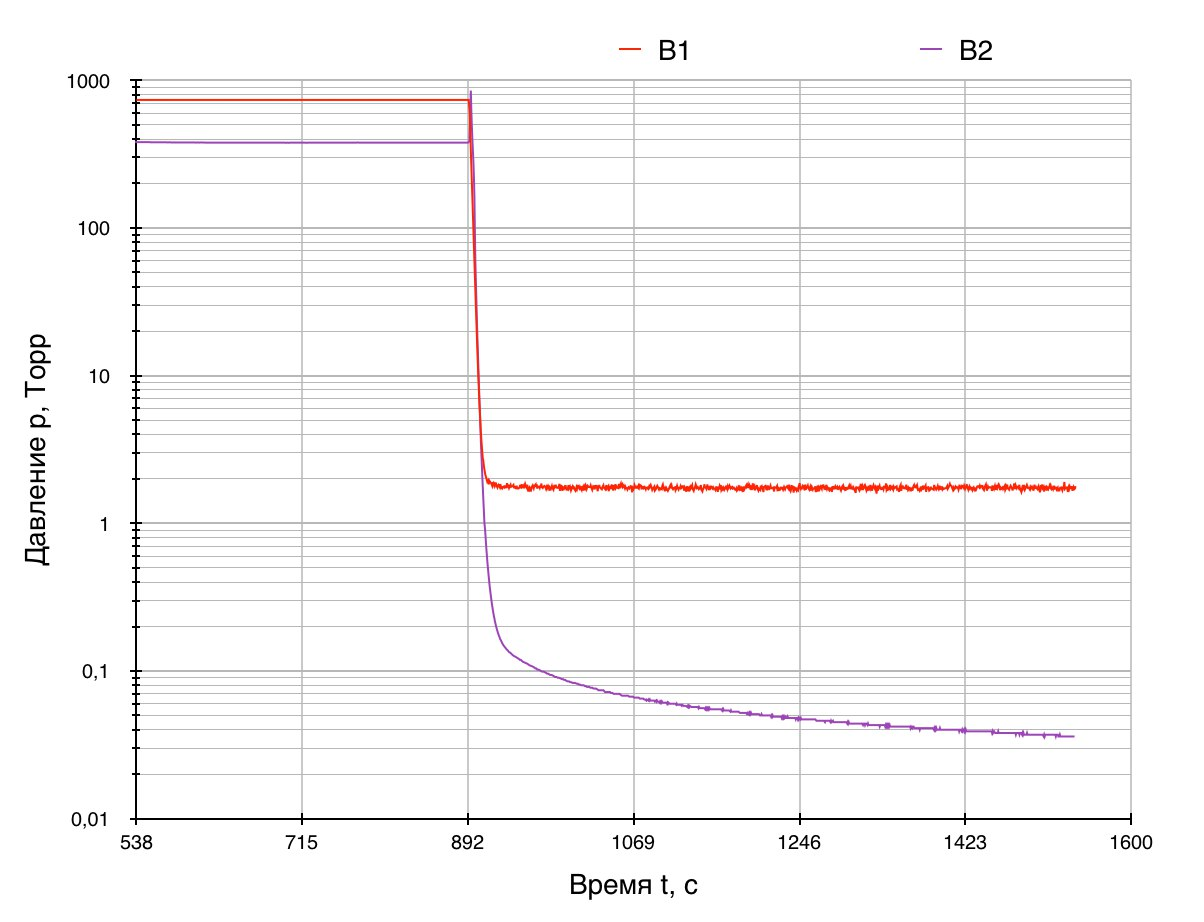
\includegraphics[width=10cm]{b1_b2.jpg}
    \caption{Зависимость показаний давления в форвакуумной части установки от времени}
    \label{fig:vac}
\end{figure}

На графике можно выявить оссобенности ёмкостного и терморезисторного вакуумметров:
\begin{enumerate}
\item Перед началом откачки воздуха из системы показания ёмкостного и терморезисторного вакуумметров отличаются: при атмосферном давлении 760 Торр ёмкостной вакуумметр показывает значение ~ 760 Торр, в то время как терморезисторный ~ 380 Торр. Делаем вывод, что вакуумметр ёмкостного типа применим для измерения давлений ~$10^2$ Торр, а терморезисторного типа определяет давление этого порядка неточно.
\item После включения форвакуумного насоса показания ёмкостного вакуумметра сразу стали уменьшаться и быстро стабилизировались в районе 1 Торр, а у терморезисторного сначала сделали скачок вверх и медленнее стали понижаться. Это объясняется низкой инертностью ёмкостного и сравнительно высокая инертность терморезисторного вакуумметров (связана с внутренним устройством прибора)
\item Предел измерений ёмкостного вакуумметра ~ 1 Торр. Его диафрагма при этих значениях максимально деформирована, на графике появляются неровности 
\item По показаниям терморезисторного вакуумметра мы можем с большой точностью определить давление порядка ~$10^-^2$ Торр
\end{enumerate}

В паспортных данных форвакуумного насоса найдём его быстродействие при давлении 0.02 Торр: $S = 5m^3/h$. Вычислим величину газового потока натекания $Q_H$ по формуле
\begin{center}
$Q_H = SP(S)=0.02torr*5m^3/h = 0,1 torr*m^3/s$
\end{center}
Переведём в sccm:
\begin{center}
$1 torr*lit/s = 3.6 torr*m^3/h = 79.05 sccm$ => $0.1 torr*m^3/s = 2.2 sccm$
\end{center}
Величина газового потока натекания - характеристика конкретной установки, зависящая от давления в ней.

\subsection{Измерение давления в форвакуумной части установки}

Используя терморезисторный вакуумметр, снимем зависимость давления в системе от производительности форвакуумного насоса. Для этого сначала выставим на регуляторе потока величину 5 sccm, а затем будем увеличивать её с шагом 10 sccm, дожидаясь стабилизации показаний В2 (~2 минуты). На рисунке 3 представлен график зависимости давления от времени, на рисунке 4 - характер изменения потока газа от времени 
\begin{figure}[H]
    \centering
    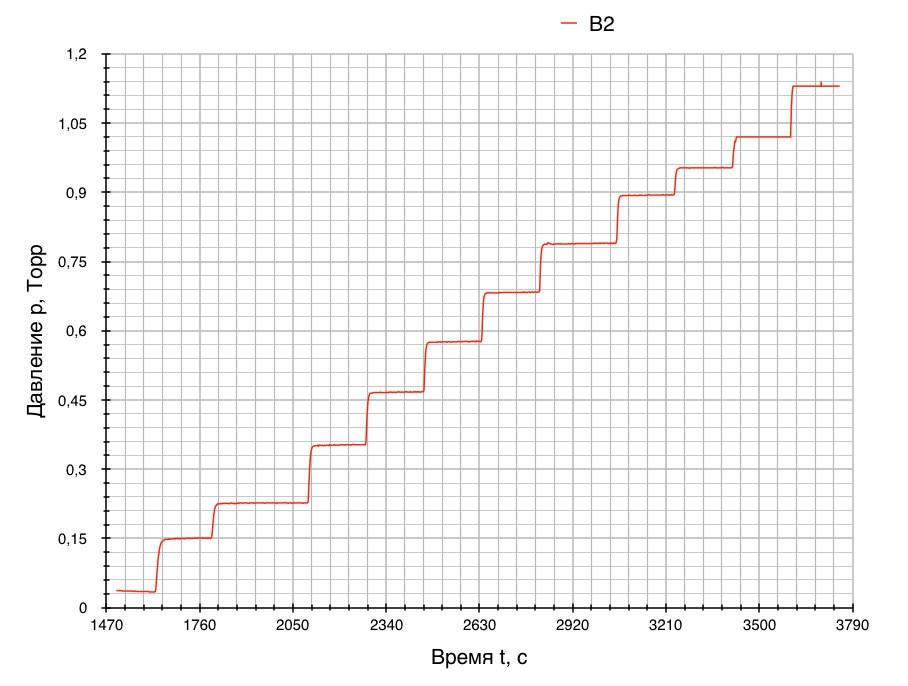
\includegraphics[width=10cm]{torr_up.jpg}
    \caption{Зависимость показаний давления в форвакуумной части установки от времени при постепенном увеличении потока воздуха}
    \label{fig:vac}
\end{figure}

\begin{figure}[H]
    \centering
    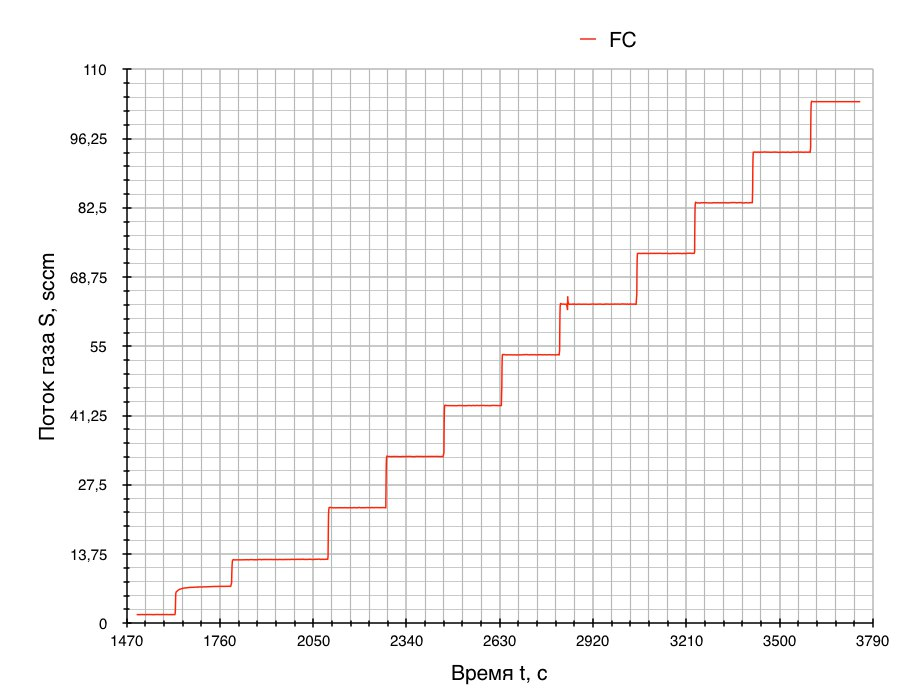
\includegraphics[width=10cm]{sccm_up.jpg}
    \caption{Зависимость потока газа через регулятор расхода от времени}
    \label{fig:vac}
\end{figure}


В таблицу 1 занесём значения установившегося давления В2 и значения соответвующих потоков через FC. В столбце $Q_F_C_s_e_t, sccm$ указаны значения, подаваемые непосредственно на регулятор расхода, $\triangle Q$ - разница между этими значениями

\begin{table}[h]
    \centering
    \begin{center}
    \caption{Величина газового потока $Q_F_C$, давление в форвакуумной части $P_2$ и скорость откачки газа $S$}
        \label{tab:my_label}
    \end{center}
   \begin{tabular}{ |p{2cm}|p{2cm}|p{2cm}|p{2cm}|p{2cm}|  }
% \multicolumn{12}{|c|}{Country List} \\
 \hline
 $Q_F_C, sccm$ & $Q_F_C_s_e_t, sccm$ & $\triangle Q, sccm$ & $P_2, torr$ & $, m^3/h$   \\
\hline

 1.73 & 0 & 1.73 & 0.041 & 1.922 \\
 7.33 & 5 & 2.33 & 0.15 & 2.225  \\
 12.66 & 10 & 2.66 & 0.227 & 2.540 \\
 22.97 & 20 & 2.97 & 0.353 & 2.963\\
 33.11 & 30 & 3.11 & 0.467 & 3.229 \\
 43.23 & 40 & 3.23 & 0.577 & 3.412 \\
 53.32 & 50 & 3.32 & 0.683 & 3.555\\
 63.37 & 60 & 3.37 & 0.789 & 3.658 \\
 73.47 & 70 & 3.47 & 0.894 & 3.743 \\
 83.55 & 80 & 3.55 & 0.953 & 3.993 \\
 93.57 & 90 & 3.57 & 1.02 & 4.178 \\
 103.6 & 100 & 3.6 & 1.13 & 4.175 \\
 \hline
\end{tabular}

\end{table}

При давлении примерно 0.02 Торр получили $\triangle Q \approx 2.2 sccm $, что по нашей оценке равно натеканию газа на нашей установке. Можно предположить, что датчик на регуляторе потока показывает значение потока сразу с учётом натекания. $Q_l_e_a_k + Q_F_C = Q$

Поток воздуха 
\begin{center}
$Q-P*S(P)=\frac{d(PV)}{dt}$
\end{center}
При $P = const$
\begin{center}
$\frac{d(PV)}{dt}=0$
\end{center}
Тогда
\begin{center}
$S(P)=\frac{Q}{P}$
\end{center}

По этой формуле рассчитаем значения S(P) и занесём результаты в таблицу 1. Построим график зависимости Q от P (рисунок 5), тогда по формуле среднее значение S будет равно угловому коэффициенту получившейся прямой, переведённой в $m^3/h$. 
\begin{center}
$S = 95.242 sccm = 4.33 m^3/h$
\end{center}

Но рассчитанные значения не совпадают с этой аппроксимацией. Значит, имеется другой характер зависимости.
Быстродействие насоса также зависит от давления в установке.

\begin{center}
$Q = \frac{d(PV)}{dt}$\\
$S(P) = \frac{Q}{P}=-V\frac{d(lnP)}{dt}$\\
$P(t) = P_0+P(0)*exp(\frac{S_0}{V}*t)$\\
$S(P) = S_0(1-\frac{P_0}{P})$
\end{center}

По значениям из таблицы 1 построим график зависимости быстродействия от давления в установке (рисунок 6). Экстраполируем его под полученную зависимость: $S_0 = 3.65 m^3/h, P_0 = 0.02 torr$. Полученное значение на 16\% отличается от экстраполированного по прямой.



\begin{figure}[H]
    \centering
    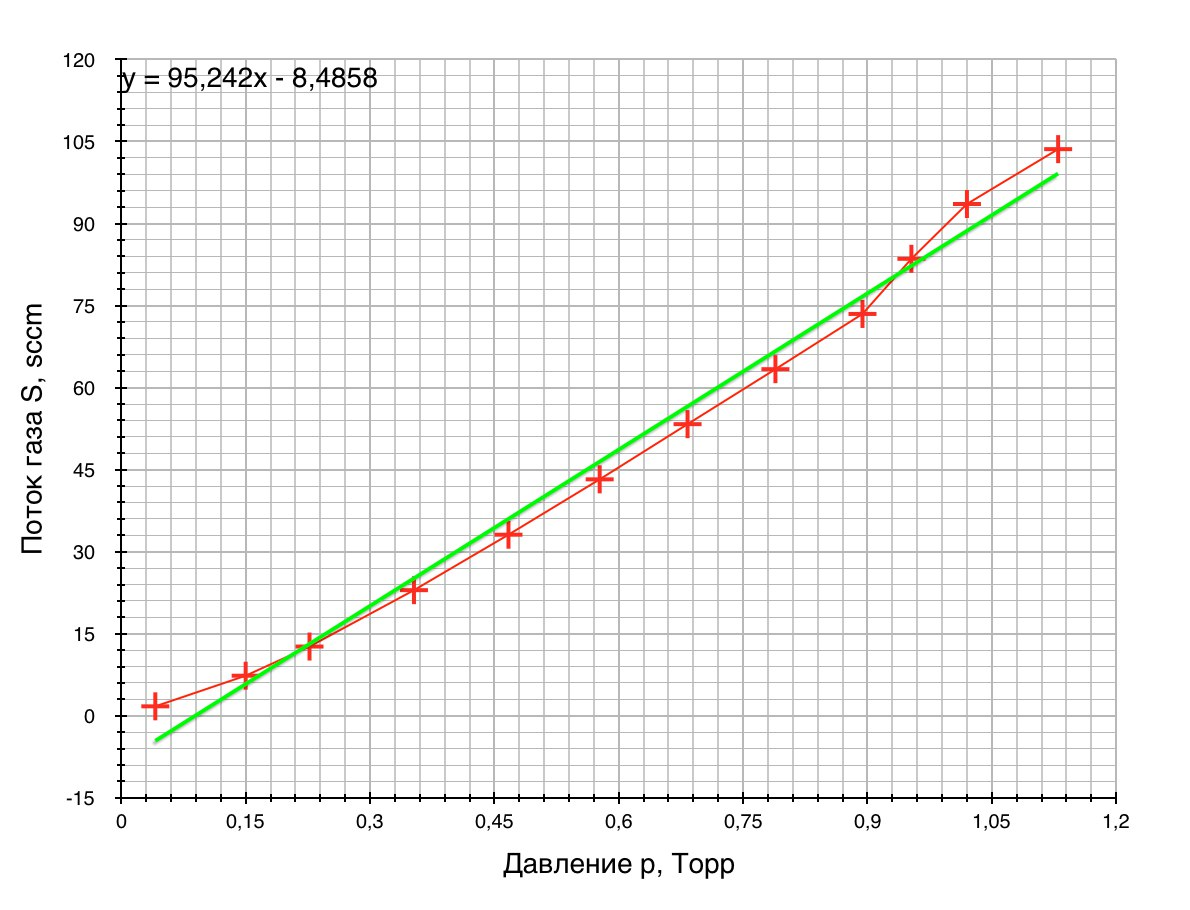
\includegraphics[width=10cm]{sccm_torr.jpg}
    \caption{Зависимость потока газа через регулятор расхода от давления}
    \label{fig:vac}
\end{figure}

\begin{figure}[H]
    \centering
    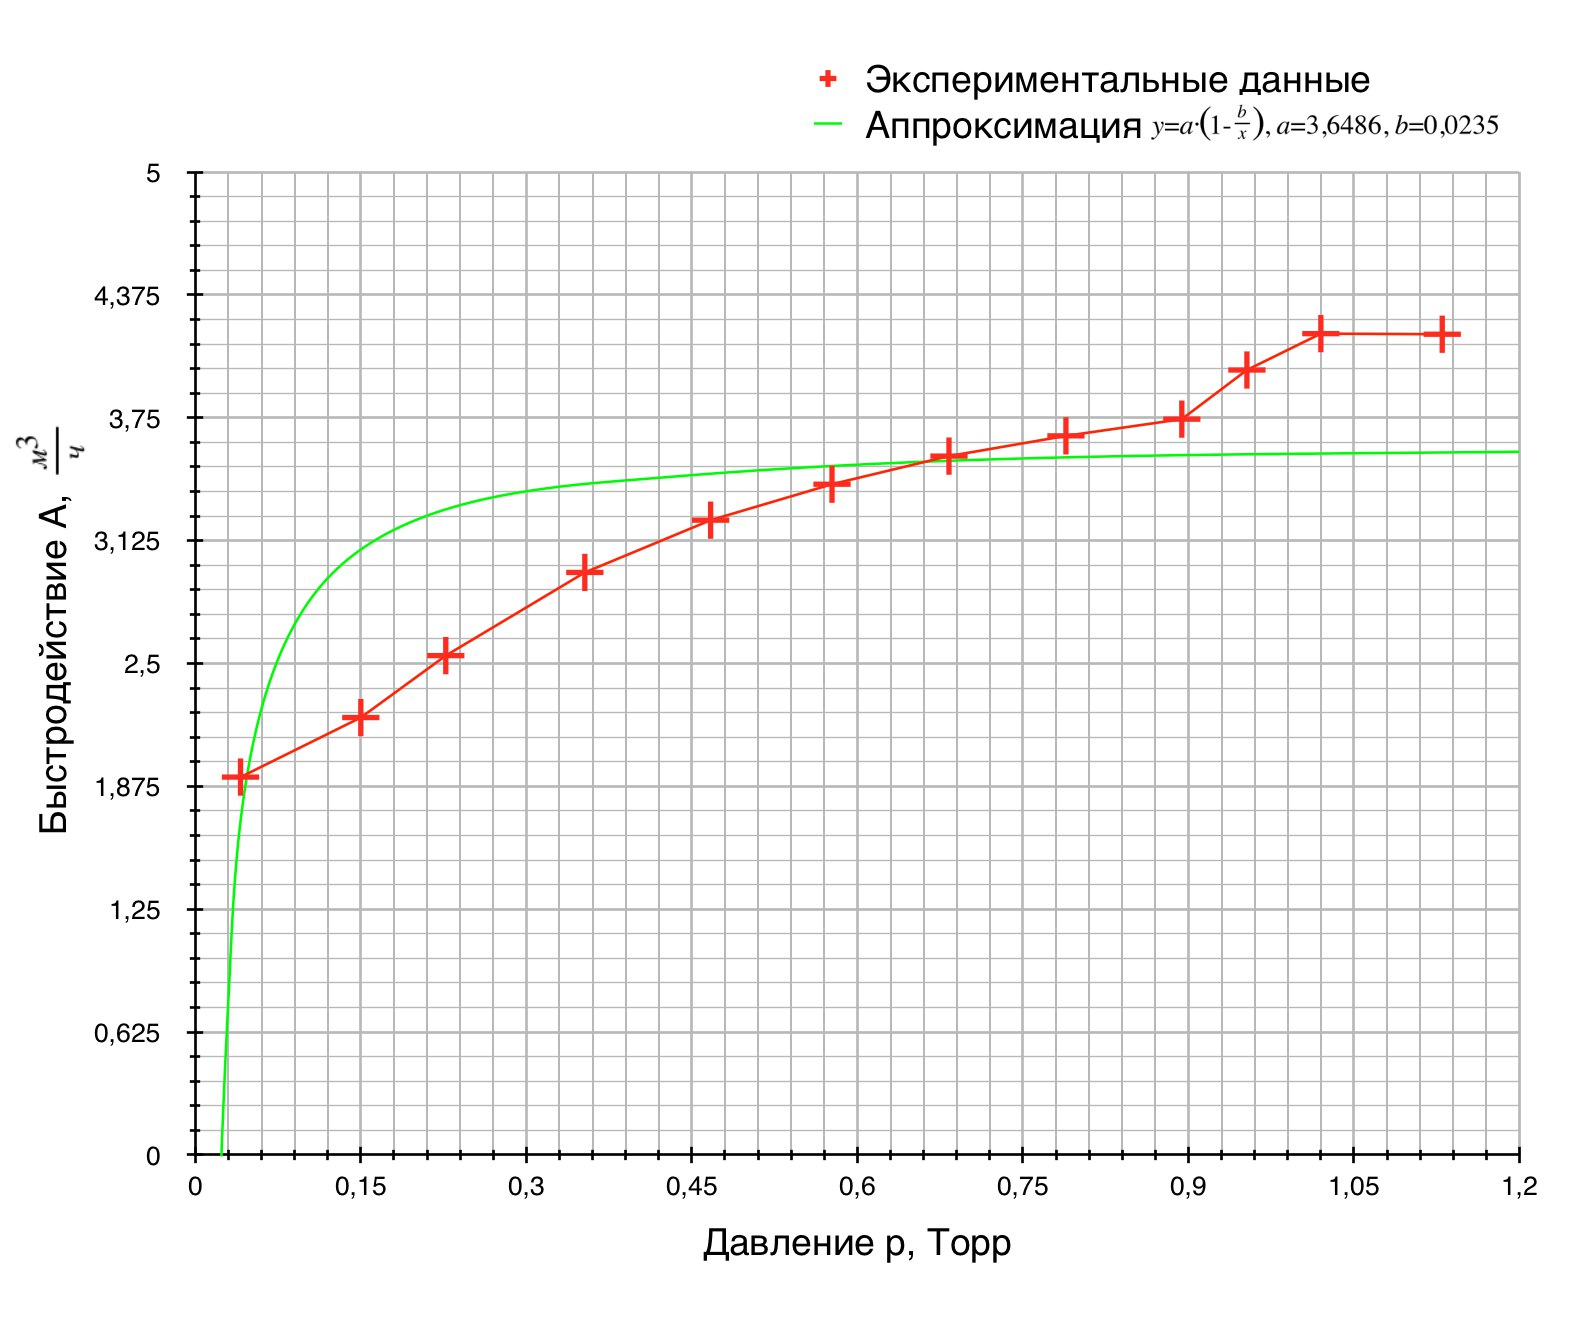
\includegraphics[width=10cm]{A_torr.jpg}
    \caption{Зависимость быстродействия форвакуумного насоса от давления в системе}
    \label{fig:vac}
\end{figure}

\subsection{Измерение производительности турбомолекулярного насоса}

\begin{enumerate}
\item Закроем К3, откроем кран К1 до появления шарика в центре ручки крана, включим турбомолекулярный насос, включим ионизационный вакуумметр, дождёмся пока вакуумметр переключит режим работы, повысив накал нити при уменьшении давления. Постепенно увеличим поток через FC до 90 sccm. Фактический поток составляет 93,5 sccm, давление в форвакуумной части 1,01 Торр.
\item Проведём снятие зависимости производительности турбомолекулярного насоса от давления. Для этого:
\begin{itemize}
  \item Перекрываем кран К2, прекращаем подачу газа через FC. Между краном К2 и диафрагмой запирается некоторое количество воздуха, давление которого соответствует давлению в форвакуумной части системы. Это давление показывает В2. Перепад давлений на диафрагме создаёт поток газа сквозь неё.
  \item Снимем зависимость показаний вакуумметров В2 и В3 от времени, графики представлены на рисунках 7 и 8
\end{itemize}  

  \begin{figure}[H]
    \centering
    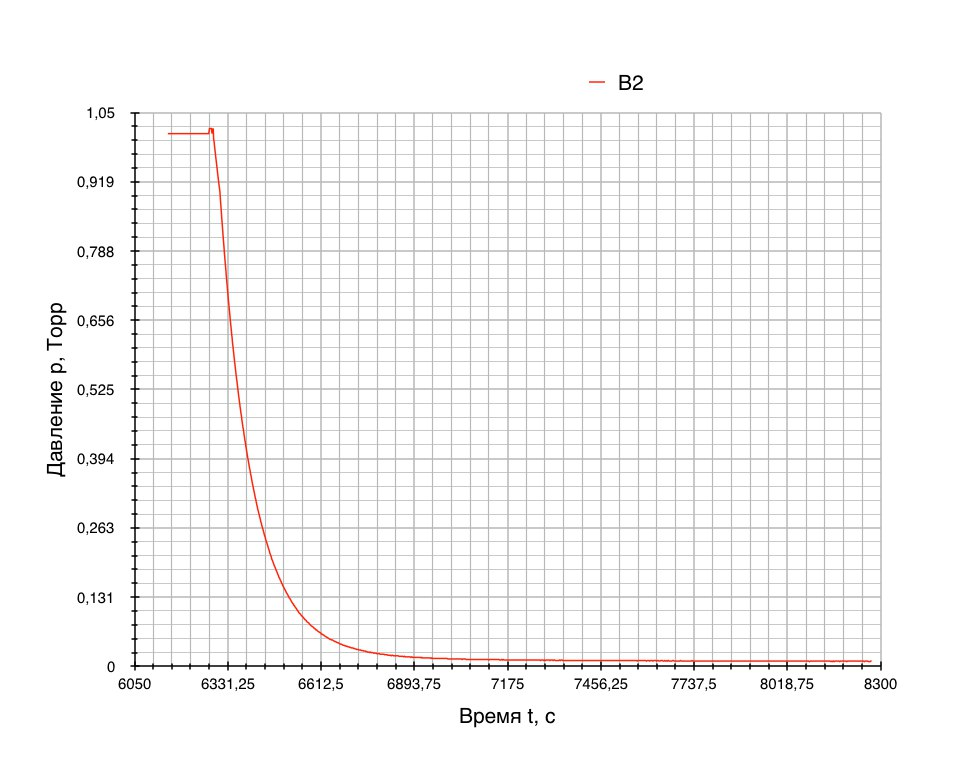
\includegraphics[width=10cm]{b2_end.jpg}
    \caption{Зависимость давления в форвакуумной части системы от времени}
    \label{fig:vac}
\end{figure}

  \begin{figure}[H]
    \centering
    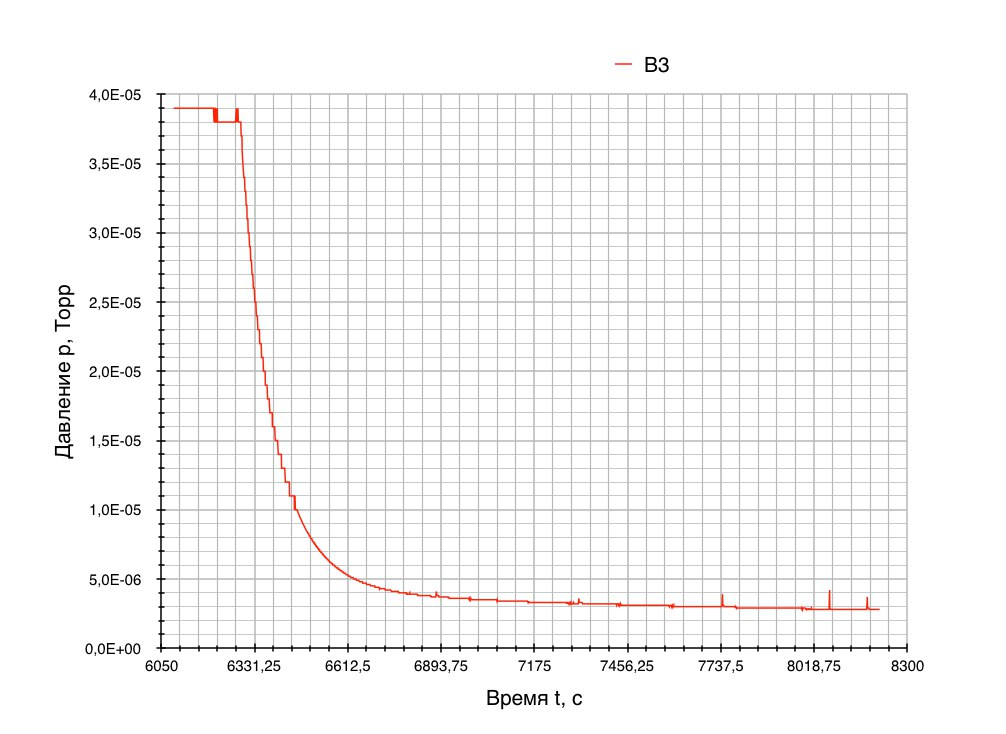
\includegraphics[width=10cm]{b3_end.jpg}
    \caption{Зависимость давления в высоковакуумной части системы от времени}
    \label{fig:vac}
\end{figure}

\item Появление скачков на рисунке 8 связано с тем, что ионизационный вакуумметр переключает режим работы, повышая накал нити при уменьшении давления.

\item Определим, можно ли считать течение газа через диафрагму молекулярным. Для этого оценим длину свободного пробега молекул:
\begin{center}
$\lambda = \frac{kT}{\sigma P} \approx 1.22m$
\end{center}
где $k = 1,38 \cdot 10^-^2^3$ Дж/К – постоянная Больцмана\\
      $T \approx 293$ К – комнатная температура\\
       $\sigma = 62,5 \cdot 10^-^2^0 m^2$ – среднее эффективное сечение рассеяния для воздуха\\
       $P \approx 4 \cdot 10^-^5$ Торр = $4 \cdot 133 \cdot 10^-^5$ Па – порядок давления в высоковакуумной части системы\\

Диаметр отверстия диафрагмы равен d = 100 мкм. Видно, что $d \ll \lambda$, поэтому течение газа через диафрагрму можно считать молекулярным. Следовательно, справедлива формула нахождения молекулярного потока через диафргаму (отверстие):
\begin{center}
$Q = S\sqrt{\frac{RT}{2\pi\mu}}(P_2-P_3)$
\end{center}
где $P_2, P_3$ - давления на В2 и В3 соответственно\\
$S = \frac{\pi d^2}{4}$ - площадь отверстия в диафрагме\\
$\mu$ - молярная масса воздуха

Так как $P_3 \\ll P_2$, формула примет вид
\begin{center}
$Q = \frac{\pi d^2}{4}\sqrt{\frac{RT}{2\pi\mu}}P_2$
\end{center}
\item Рассмортим модель потока через турбомолекулярный насос
\begin{center}
$P_3S(P_3) = Q - \frac{d(P_2V)}{dt}$\\
$Q \gg \frac{d(P_2V)}{dt}$
\end{center}
Получим:
\begin{center}
$P_3S(P_3) = Q = \frac{\pi d^2}{4}\sqrt{\frac{RT}{2\pi\mu}}P_2$
\end{center}

  \begin{figure}[H]
    \centering
    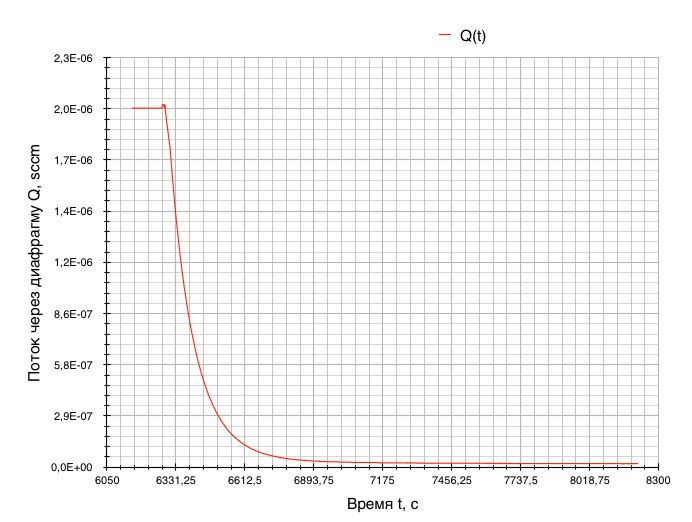
\includegraphics[width=10cm]{stream.jpg}
    \caption{Зависимость потока через турбомолекулярный насос Q от времени}
    \label{fig:vac}
\end{figure}

\item Быстродействие насоса определим через значение потока:
\begin{center}
$Q = P_3S(P)$
\end{center}
Пользуясь тем, что производительность можно считать постоянной в некоторой области при установившемся давлении, найдём её из отношения потока к давлению. Для этого воспользуемся графиком, представленным на рис. 9
  \begin{figure}[H]
    \centering
    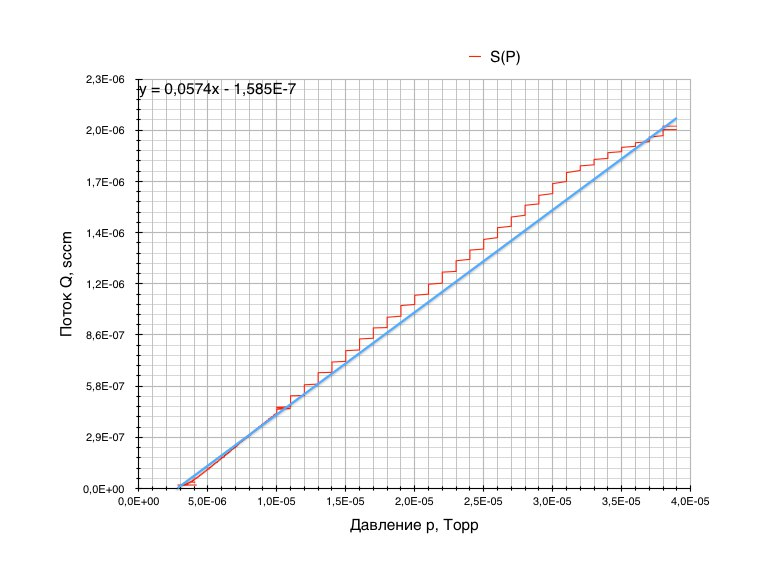
\includegraphics[width=10cm]{productivity.jpg}
    \caption{Зависимость потока через ТМН от давления в системе для определения производительности ТМН}
    \label{fig:vac}
\end{figure}

Здесь значение производительности будет угловым коэффициентом аппроксисирующей прямой:
$S = 0.0574 sccm/2.2 = 0.0261 m^3/s = 26.1$ л/с

\item Сравним это значение с данными производителя: график зависимости производительности от давления при разных газах представлен на рисунке 10
  \begin{figure}[h]
    \centering
    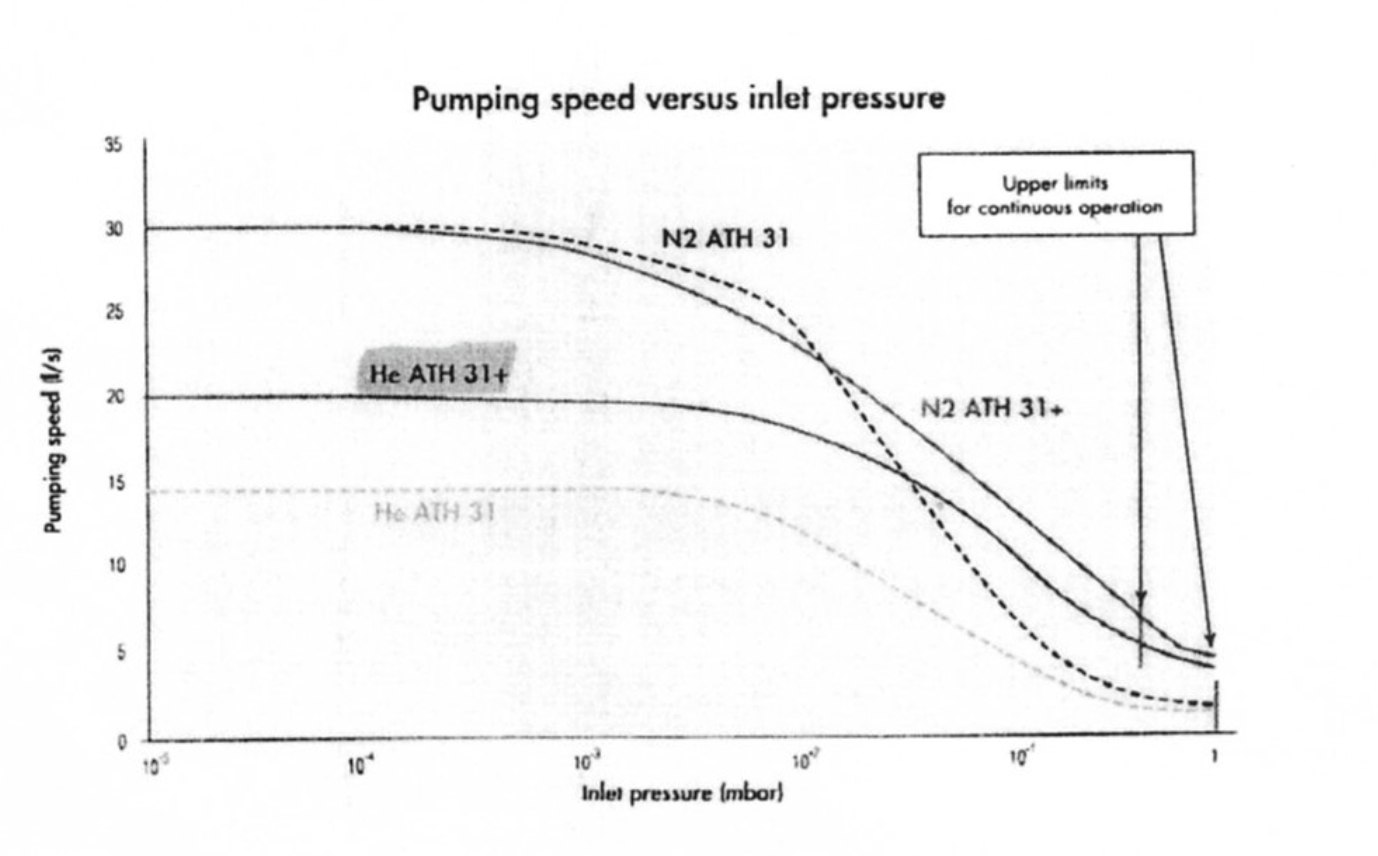
\includegraphics[width=10cm]{man_data.jpg}
    \caption{Данные производителя о зависимости производительности тМН от давления}
    \label{fig:vac}
\end{figure}

По документации производительность ТМН, перекачивающего азот (основная часть атмосферы), равна 30 л/с при давлениях порядка $10^-^5$ Торр и практически постоянна. Турбомолекулярный насос в нашем эксперименте быстро вышел на свои предельные значения при $10^-^5$ Торр и рассчитанная производительность практически совпадает с данными производителя.

\item Для определения объёма рабочей камеры необходимо создать условия отсутствия натекания газа через диафрагму. В нашем эксперименте таких условия предоставлено не было, следовательно, нельзя с большой точность определить объём рабочей камеры
\end{enumerate}

\section {Вывод}
В ходе работы мы ознакомились с принципами работы вакуумной техники, определили характеристики насосов и вакуумметров, изучили методы получения и измерения вакуума. 
\begin{enumerate}
\item Определены рабочие диапазоны вакуумметров:
\begin{itemize}
  \item ёмкостной:$760 - 1$ Торр
  \item терморезисторный: $10 - 10^-^3 $ Торр
  \item ионизационный: $10^-^3 - 10^-^5$ Торр
\end{itemize}
\item На установке получен высокий вакуум порядка $10^-^5$ Торр
\item Определены быстродействия вакуумных насосов:
\begin{itemize}
  \item форвакуумный: $3.65 m^3/h$
  \item турбомолекулярный $26.1 m^3/h$: 
\end{itemize}
\end{enumerate}

\section{Список использованной литературы}
\begin{enumerate}
\item Методы получения высокого вакуума: лабораторная работа по курсу Вакуумная электроника / сост.: А.С. Батурин, И.Н. Ескин, Д.А. Свинцов, П.А. Стариков, Е.П. Шешин – М.: МФТИ, 2010. – 36 с.
\item Шешин Е.П. — Основы вакуумной электроники: учеб. пособие. – 2-е издание, испр. И доп. - М.: МФТИ, 2009.  - 149 с.
\item Шешин Е.П. — Вакуумные технологии: учеб. пособие. / 
Долгопрудный: издательский Дом «Интеллект», 2009.  - 504 с.
\end{enumerate}



\end{document}
